      
               
                \begin{ledgroupsized}[r]{120mm}
                \footnotesize 
                \pstart                
                \noindent\textbf{\"{U}berlieferung:}   
                \pend
                \end{ledgroupsized}
            
              
                            \begin{ledgroupsized}[r]{114mm}
                            \footnotesize 
                            \pstart \parindent -6mm
                            \makebox[6mm][l]{\textit{L}}Konzept: LH XXXVII 3 Bl. 95\textendash 96. 1 Bog. 2\textsuperscript{o}. 1 1/4 S., zweispaltig. Bl. 96~r\textsuperscript{o}  und 1/4 von Bl. 96 v\textsuperscript{o} unser Text. Linke Spalte auf Bl. 96 r\textsuperscript{o} fortlaufender Text, rechts Rechnungen und Zeichnungen. Bl. 95 sowie der gr\"{o}ßere Teil von Bl. 96 v\textsuperscript{o} zu N.~39 geh\"{o}rend. Papierverluste an den Seitenr\"{a}ndern, jedoch kaum Textverluste. Auf Bl. 96 r\textsuperscript{o} eine unvollst\"{a}ndige und gestrichene Zeichnung, die als erster Versuch von \textit{[Fig. 1]} im Druck nicht wiedergegeben wird.\\Cc 2, Nr. 486 A tlw.\pend
                            \end{ledgroupsized}
                %\normalsize
                \vspace*{5mm}
                \begin{ledgroup}
                \footnotesize 
                \pstart
            \noindent\footnotesize{\textbf{Datierungsgr\"{u}nde}: Der Text dieses St\"{u}cks befindet sich zusammen mit Textteilen von N.~39 auf einem Bogen. Aus dem Schriftbefund geht hervor, dass unser St\"{u}ck entweder vor der Abfassung von N. 39 vorhanden gewesen sein muss oder gleichzeitig damit entstand. Da sich beide Texte inhaltlich ber\"{u}hren, gehen wir von einem gemeinsamen Entstehungszeitraum aus und \"{u}bernehmen die Datierung aus N. 39.}
                \pend
                \end{ledgroup}
            
                \vspace*{8mm}
                \pstart 
                \normalsize
            [96 r\textsuperscript{o}] \edtext{Constat siphonem bicrurum \pgrk{<eterom'hqh}, aqua plenus altero crure breviore in aquam vase quodam contentam intrantem, altero corpore extra vas descendentem,}{\lemma{}\Afootnote{ \textit{ (1) }\ Galilaeus\protect\index{Namensregister}{\textso{Galilei} (Galilaeus, Galileus), Galileo 1564\textendash 1642|textit} \textit{ (2) }\ Galilaeum\protect\index{Namensregister}{\textso{Galilei} (Galilaeus, Galileus), Galileo 1564\textendash 1642|textit} memo \textit{ (3) }\ Recepta fuit sententia in scholis effectus quosdam extraordinarios naturae, qui scilicet eveniunt, quoties alioquin corpore uno ex suo loco exeunte, aliud sensibile intrare non posset; a \textso{fuga Vacui }\protect\index{Sachverzeichnis}{fuga vacui|textit}oriri, ut quod duae Tabulae politae\protect\index{Sachverzeichnis}{tabulae!politae|textit} cohaerent; \textit{(a)}\ quod aqua \textit{(b)}\ quod liquor ex vase non effluit, cujus unum tantum foramen apertum est, quod \textit{(c)}\  quod corpore uno \textbar\ ex loco quodam \textit{ erg.}\ \textbar\  extracto proximum invita etiam gravitate\protect\index{Sachverzeichnis}{gravitas|textit} sua succedere cogitur (ut aere ex tubo quodam exucto globulum plumbeum in fundo positum prorumpere, et Embolo\protect\index{Sachverzeichnis}{embolus|textit} extracto aquam in antliam\protect\index{Sachverzeichnis}{antlia|textit} assurgere constat) quod Sipho\protect\index{Sachverzeichnis}{sipho|textit} bicrurus altero crure in aquam vase quodam contentam intrans, altero \textit{(aa)}\ infra \textit{(bb)}\ vasis \textit{(cc)}\ aquae superficiem \textit{(dd)}\ corpore extra vas descendens. \textit{ (4) }\ Constat siphonem bicrurum \pgrk{<eterom'hqh}, [...] descendentem, \textit{ L}}} aquam ex vase \edtext{elicere}{\lemma{vase}\Afootnote{ \textit{ (1) }\ elici facit, donec \textit{ (2) }\ effluere facit \textit{ (3) }\ elicere \textit{ L}}}, donec superficies aquae ad \edtext{orificium}{\lemma{ad}\Afootnote{ \textit{ (1) }\ eundem cum \textit{ (2) }\ orificium \textit{ L}}} usque cruris extra vas positi decreverit. \edtext{Hujus}{\lemma{decreverit.}\Afootnote{ \textit{ (1) }\ Ex quo \textit{ (2) }\ Cujus postremi \textit{ (3) }\ Hujus \textit{ L}}}  phaenomeni ope \edtext{rationem}{\lemma{ope}\Afootnote{ \textit{ (1) }\ , ut obiter hoc loco exponam, aliquando \textit{ (2) }\ rationem \textit{ L}}} inveni conficiendi clepsydram\protect\index{Sachverzeichnis}{clepsydra} uniformiter fluentem. Constat veteres clepsydris\protect\index{Sachverzeichnis}{clepsydra}, aquam scilicet extillantibus fuisse usos. Sed cum \edtext{celeritas effluxus, decrescente continuo altitudine,}{\lemma{cum}\Afootnote{ \textit{ (1) }\ Clepsydra\protect\index{Sachverzeichnis}{clepsydra|textit} initio fortius flueret, \textit{ (2) }\ celeritas effluxus, decrescente continuo altitudine, \textit{ L}}} ac proinde pressione aquae continuo diminueretur, \edtext{nec proinde satis ad tempus mensurandum uniformis esset}{\lemma{diminueretur,}\Afootnote{ \textit{ (1) }\ necesse erat rotas\protect\index{Sachverzeichnis}{rota|textit} horarum dividere in partes inaequales, quod nec commode applicari poterat ad \textit{(a)}\ minuta \textit{(b)}\ partes horae minutiores \textit{ (2) }\ nec [...] esset \textit{ L}}} Horologiis\protect\index{Sachverzeichnis}{horologium} arenariis uti placuit, in quibus incommodum quidem idem at non aeque sensibile. Ego considerato siphonis\protect\index{Sachverzeichnis}{sipho} istius bicruri effectu hoc machinamentum \edtext{clepsydrae\protect\index{Sachverzeichnis}{clepsydra} uniformis}{\lemma{}\Afootnote{clepsydrae\protect\index{Sachverzeichnis}{clepsydra} uniformis \textit{ erg.} \textit{ L}}} commentus sum.
            \pend \vspace{2.0ex}
               \begin{center}
               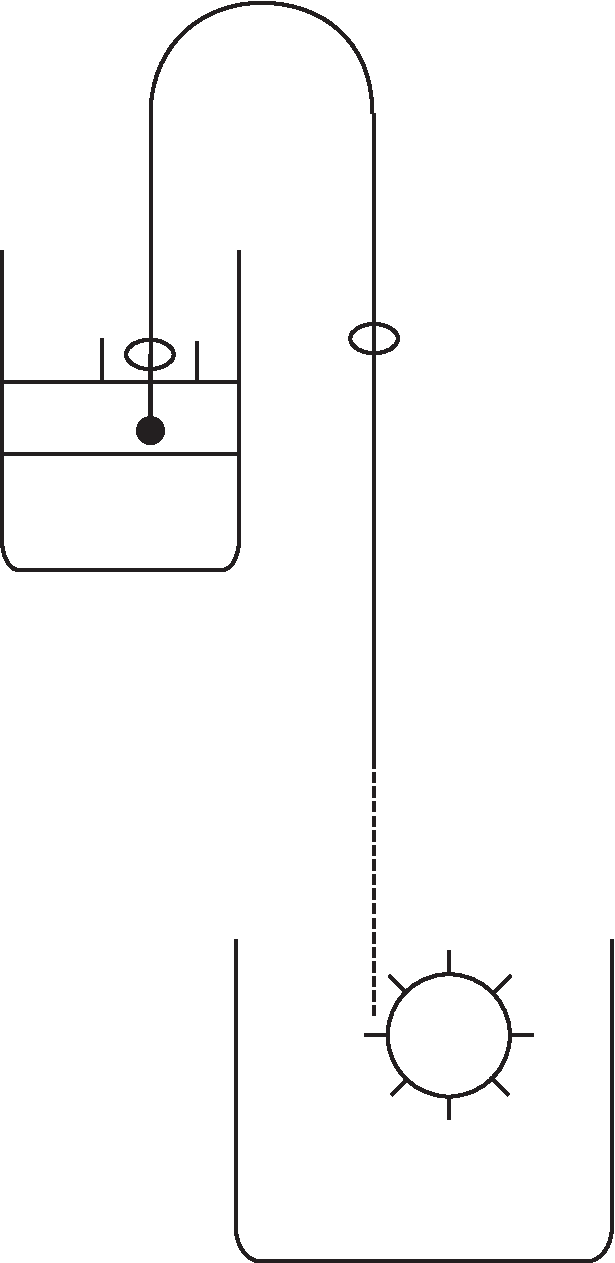
\includegraphics[width=0.3\textwidth]{images/37_3_96r2.pdf}
               \\ \textit{[Fig. 1]}
               \end{center}
               \newpage
               \begin{center}
               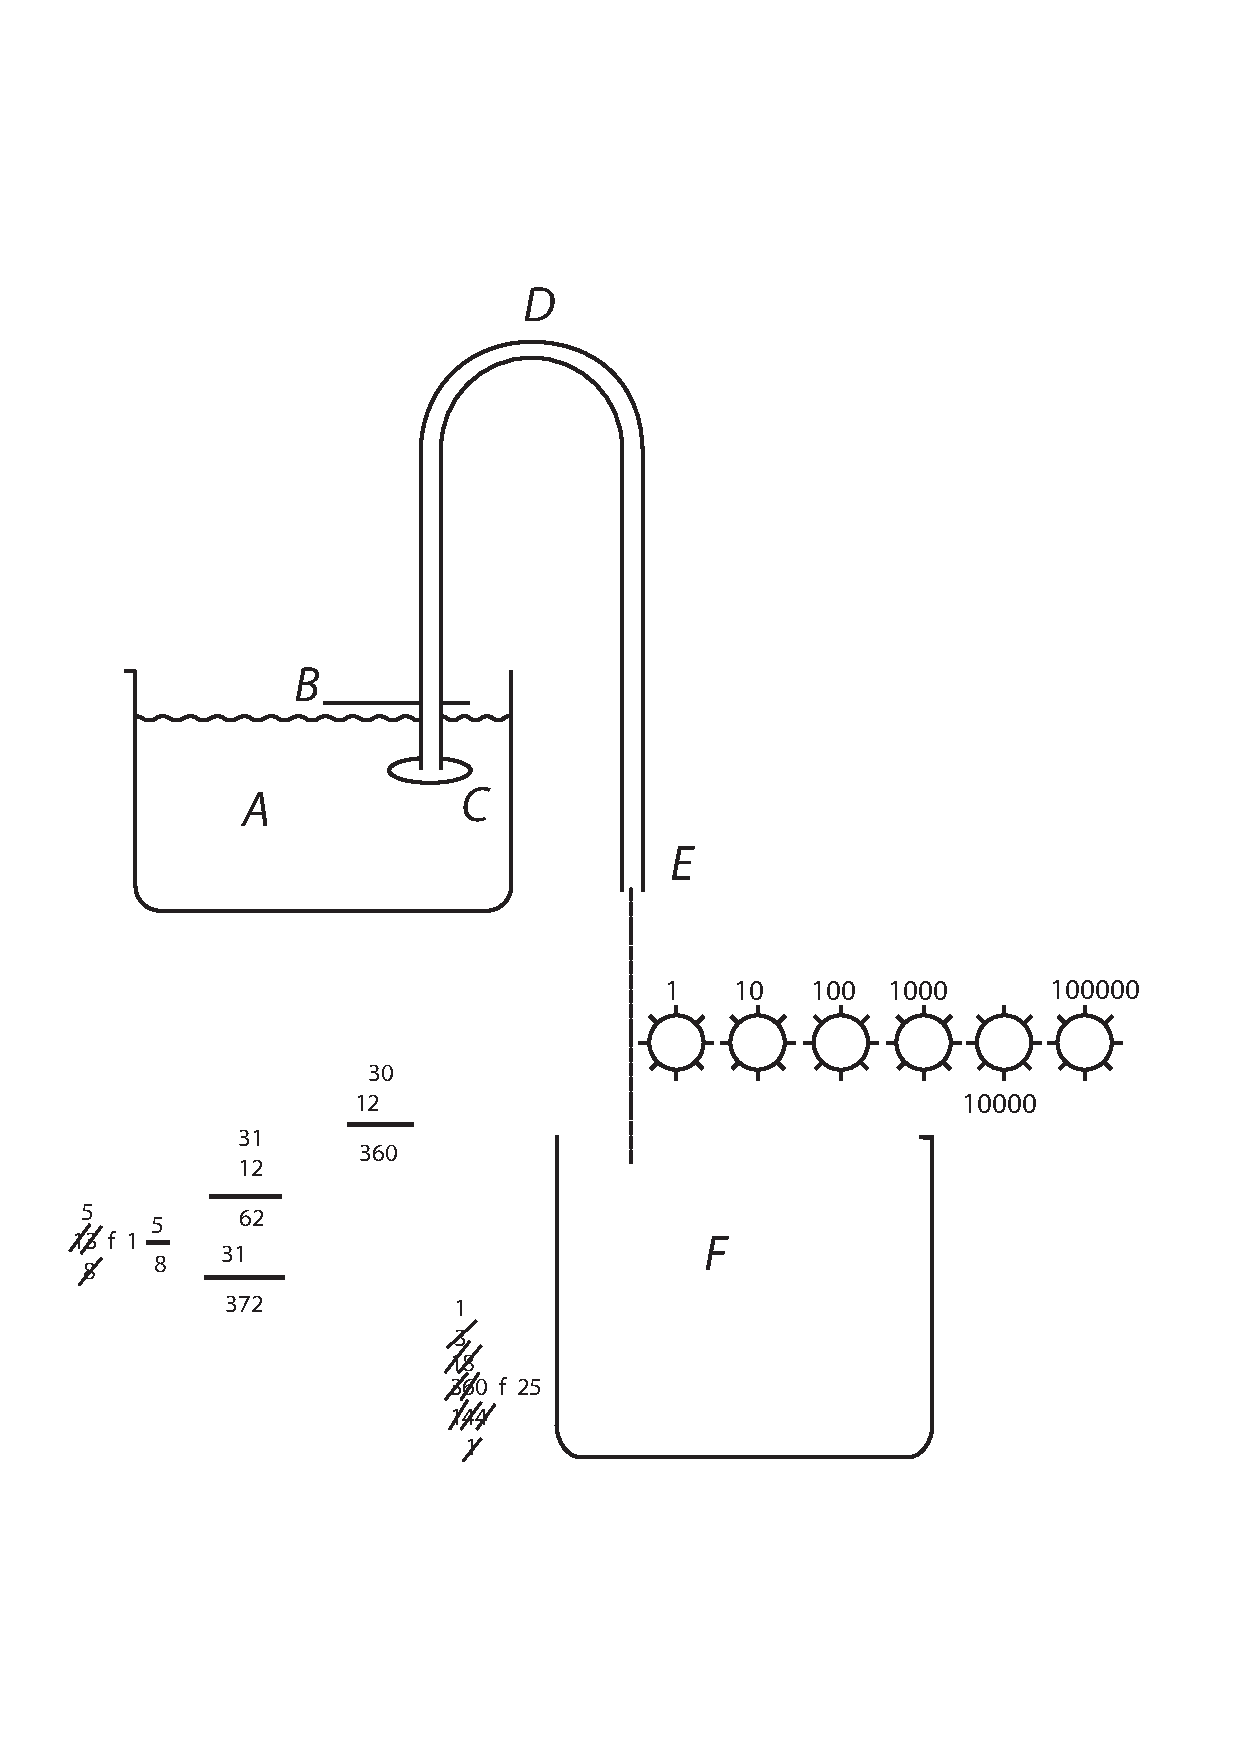
\includegraphics[width=0.7\textwidth]{images/37_3_96r1.pdf}
               \\ \textit{[Fig. 2]}\\
               \end{center}
           \pstart\textit{Nebenrechnungen zu [Fig. 2]}:\\
              $\protect\begin{array}{r} \hspace{5.5pt}5\\\cancel{1}\cancel{3}\\\hspace{5.5pt}\cancel{8}\protect\end{array}$ $\protect\begin{array}{l}f\hspace{5.5pt}1\protect\displaystyle\protect\frac{5}{8}\protect\end{array}$
            \hspace{10mm} $\protect\begin{array}{r} 31\\12\\\overline{62}\\31\\\overline{[372]}\protect\end{array}$ \hspace{10mm} $\protect\begin{array}{l} \hspace{5.5pt}30\\12\\\overline{360}\protect\end{array}$\hspace{10mm} $\protect\begin{array}{l} 1\\\cancel{3}\\\cancel{1}\cancel{8}\\\cancel{3}\cancel{6}\cancel{0}\hspace{5.5pt}f\hspace{5.5pt}25\\\cancel{1}\cancel{4}\cancel{4}\\~~\cancel{1}\protect\end{array}$\edtext{}{\lemma{}\Afootnote{373\textit{\ L \"{a}ndert Hrsg.}}}
            \pend
            \pstart \edtext{Esto vas \textit{A} aquam continens, sipho bicrurus \textit{CDE} cujus crus minus \textit{DC} intret in aquam vasis \textit{A} et orificio \textit{C} prope attingat fundum vasis. Crus majus \textit{DE} orificio \textit{E} descendat infra \textit{C}.}{\lemma{}\Afootnote{\textit{ (1) }\ Clepsydram\protect\index{Sachverzeichnis}{clepsydra|textit} uniformem inde praeberi sic ostendo: \textit{(a)}\ cum \textit{(b)}\ rationem inveni facilem \textit{ (2) }\ Esto \textit{(a)}\ in vase \textit{(b)}\ vas \textit{A} aquam \hspace{2mm}continens, \textit{(aa)}\ in quod \hspace{2mm}intret \textit{(bb)}\ sipho [...] \hspace{2mm}minus  \textbar\ \textit{DC} \textit{ erg.}\ \textbar\  intret in aquam vasis \textit{A} \textit{(aaa)}\ prope ad fundum crus min \textit{(bbb)}\ et [...] \textit{C}.  \textit{ erg.} \textit{ L}}}
             \pend
             \pstart \edtext{Esto vas aquam continens \textit{A} in aquae superficie natans Tabula levis \textit{B} cui infixus sipho bicrurus \textit{CDE} cujus crus minus \textit{CD} per mediam Tabulam cui infixum est descendit attingit aquam in \textit{C} alterum crus majus \textit{DE} extra aquam usque ad \textit{E} infra fundum vasis \textit{A}.}{\lemma{}\Afootnote{Esto [...] Tabula  \textit{ (1) }\ lignea \textit{ (2) }\ levis [...] crus  \textbar\ minus \textit{ erg.}\ \textbar\ \textit{CD} [...] descendit \textit{(a)}\ in aquam usque superficiem \textit{(b)}\ in aquam usque ad C. \textit{(c)}\ attingit [...] vasis  \textbar\ \textit{A} \textit{ erg.}\ \textbar\ . \textit{ gestr. und wieder g\"ultig gemacht} \textit{ L}}} Esto vero et crassities siphonis\protect\index{Sachverzeichnis}{sipho} et apertura utrobique aequalis tum in \textit{C} tum in \textit{E}. 
            Sipho\protect\index{Sachverzeichnis}{sipho} aqua impleatur, sive jam ante \edtext{immissa}{\lemma{ante}\Afootnote{ \textit{ (1) }\ infusa \textit{ (2) }\ immissa \textit{ L}}}, antequam aquae vasis \textit{A} innatet, \edtext{orificiis}{\lemma{innatet,}\Afootnote{ \textit{ (1) }\ sive orificia \textit{ (2) }\ orificiis \textit{ L}}} interim \edtext{obturatis,}{\lemma{}\Afootnote{interim  \textbar\ digito \textit{ gestr.}\ \textbar\ obturatis, \textit{ L}}} ne effluat antequam opus sit; vel suctu \edtext{oris}{\lemma{suctu}\Afootnote{ \textit{ (1) }\ ex aqua \textit{ (2) }\ oris \textit{ L}}} in \textit{C} applicati ex vase \textit{A} attracto. Quo facto aqua destillabit ex \textit{E} in subjectum vas \textit{F} novaque continue aqua in siphonem\protect\index{Sachverzeichnis}{sipho} succedet, donec scilicet \edtext{superficies effluxu deminuta descendat infra \textit{C}.}{\lemma{scilicet}\Afootnote{ \textit{ (1) }\ orificium cruris longioris \textit{E} \textit{ (2) }\ aquae in vase \textit{A} continuo effluxu deminuta descendat usque ad orificium cruris longioris \textit{E} \textit{ (3) }\ aquae in vase \textit{A}  effluxu deminuta descendat infra \textit{C} \textit{ (4) }\ superficies \textit{(a)}\ aquae in vase \textit{A} effluxu aquae dimin \textit{(b)}\ effluxu deminuta descendat infra \textit{C}. \textit{ L}}} \edtext{Et hoc quidem fieret, si sipho\protect\index{Sachverzeichnis}{sipho} immobilis interim esset, verum quia sipho\protect\index{Sachverzeichnis}{sipho} aquae innatat una cum Tabula cui infixus est, descendet et ipse cum orificio \textit{E} quantum descendit aquae superficies. Nunquam ergo aquae superficies orificium \textit{C} deseret ac proinde nunquam cessabit extillatio.}{\lemma{}\Afootnote{Et hoc [...] orificio \textit{E} \textit{ (1) }\ nunquam ergo cessabit \textit{(a)}\ effluxus \textit{(b)}\  extillatio, donec \textit{(aa)}\ omnis aq \textit{(bb)}\ vase \textit{A} omni \textbar\ pene \textit{ erg.}\ \textbar\  aqua exhausto orificium \textit{C} fundum ipsum vasis attingat. \textit{ (2) }\ quantum [...] orificium \textit{(a)}\ \textit{E} assequetur \textit{(b)}\ \textit{C} [...] extillatio. \textit{ gestr. und wieder g\"ultig gemacht} \textit{ L}}} Cumque sipho\protect\index{Sachverzeichnis}{sipho} \edtext{interim}{\lemma{}\Afootnote{interim \textit{ erg.} \textit{ L}}} semper sit plenus, \edtext{et altitudo aquae super \textit{C} eminentis, quae sola in siphonem\protect\index{Sachverzeichnis}{sipho} premere posset, semper eadem, ergo}{\lemma{}\Afootnote{et altitudo aquae super \textit{C} eminentis, quae sola in siphonem\protect\index{Sachverzeichnis}{sipho} premere posset, semper eadem, ergo \textit{ erg.} \textit{ L}}} pressio aquae semper eadem, ac proinde extillatio aequalis erit. Quod desiderabatur. Destillatio ergo  guttarum tempus exacte mensurabit\edtext{. Ausim dicere post penduli vibrationes nihil}{\lemma{mansurabit}\Afootnote{ \textit{ (1) }\ , ac proinde ita ut post penduli vibrationes\protect\index{Sachverzeichnis}{vibratio penduli|textit} nihi \textit{ (2) }\ . Ausim dicere post penduli vibrationes nihil \textit{ L}}} nobis suppetere exactius. 
            \edtext{Et}{\lemma{exactius.}\Afootnote{ \textit{ (1) }\ Nam  \textit{ (2) }\ Et \textit{ L}}} quemadmodum penduli\protect\index{Sachverzeichnis}{pendulum} cursus non cessat, etiam eo tempore quo Horologium\protect\index{Sachverzeichnis}{horologium} tenditur \edtext{nec fit}{\lemma{tenditur}\Afootnote{ \textit{ (1) }\ ita \textit{ (2) }\ quod \textit{ (3) }\ qua praerogativa omnia alia \textit{ (4) }\ nec fit \textit{ L}}} irregularis etsi Elaterium\protect\index{Sachverzeichnis}{elaterium} cui applicatur mature serove, \edtext{item}{\lemma{serove,}\Afootnote{ \textit{ (1) }\ an \textit{ (2) }\ item \textit{ L}}} fortiter aut debiliter tendatur; nec turbatur, etsi Elaterium\protect\index{Sachverzeichnis}{elaterium} nunc celerius nunc tardius se restituat, et tractu temporis debilitetur, quae \edtext{praerogativae}{\lemma{}\Afootnote{praerogativae \textit{ erg.} \textit{ L}}} nulli hactenus invento horologio\protect\index{Sachverzeichnis}{horologium} tribui potuere; ita in hoc Horologio\protect\index{Sachverzeichnis}{horologium} eadem evenire necesse est. Nam si aquam vel manu vel machina non difficulter applicanda ex vase \textit{F} in vas \textit{A} refundas, antequam totum exhaustum sit, \edtext{restituetur Horologium\protect\index{Sachverzeichnis}{horologium} in priorem statum, et}{\lemma{}\Afootnote{restituetur Horologium\protect\index{Sachverzeichnis}{horologium} in priorem statum, et \textit{ erg.} \textit{ L}}} non ideo minus interim continuabitur \edtext{extillatio}{\lemma{continuabitur}\Afootnote{ \textit{ (1) }\ distillatio eodem \textit{ (2) }\ extillatio \textit{ L}}}, eodem plane modo: pressio enim non perturbatur quia aqua \edtext{vasis \textit{A}}{\lemma{}\Afootnote{vasis \textit{A} \textit{ erg.} \textit{ L}}} aucta seu superficie ejus ascendente, etiam Tabula \textit{B} ascendet cum toto siphone\protect\index{Sachverzeichnis}{sipho}. \edtext{Ut res}{\lemma{siphone.}\Afootnote{ \textit{ (1) }\ Ut experimentum \textit{ (2) }\ Ut res \textit{ L}}} succedat rectius, \edtext{opus est}{\lemma{rectius,}\Afootnote{ \textit{ (1) }\ necesse est \textit{ (2) }\ opus est \textit{ L}}} siphonem\protect\index{Sachverzeichnis}{sipho} sustineri ne extra vas labatur, Tabulam \textit{B}. esse satis levem, ut siphonem\protect\index{Sachverzeichnis}{sipho} possit \edtext{ferre}{\lemma{possit}\Afootnote{ \textit{ (1) }\ sustinere \textit{ (2) }\ ferre \textit{ L}}}, 